\documentclass[]{book}
\usepackage{lmodern}
\usepackage{amssymb,amsmath}
\usepackage{ifxetex,ifluatex}
\usepackage{fixltx2e} % provides \textsubscript
\ifnum 0\ifxetex 1\fi\ifluatex 1\fi=0 % if pdftex
  \usepackage[T1]{fontenc}
  \usepackage[utf8]{inputenc}
\else % if luatex or xelatex
  \ifxetex
    \usepackage{mathspec}
  \else
    \usepackage{fontspec}
  \fi
  \defaultfontfeatures{Ligatures=TeX,Scale=MatchLowercase}
\fi
% use upquote if available, for straight quotes in verbatim environments
\IfFileExists{upquote.sty}{\usepackage{upquote}}{}
% use microtype if available
\IfFileExists{microtype.sty}{%
\usepackage{microtype}
\UseMicrotypeSet[protrusion]{basicmath} % disable protrusion for tt fonts
}{}
\usepackage[margin=1in]{geometry}
\usepackage{hyperref}
\hypersetup{unicode=true,
            pdftitle={联信'自呼机器人` REST API},
            pdfauthor={联信策略中心},
            pdfborder={0 0 0},
            breaklinks=true}
\urlstyle{same}  % don't use monospace font for urls
\usepackage{natbib}
\bibliographystyle{apalike}
\usepackage{longtable,booktabs}
\usepackage{graphicx,grffile}
\makeatletter
\def\maxwidth{\ifdim\Gin@nat@width>\linewidth\linewidth\else\Gin@nat@width\fi}
\def\maxheight{\ifdim\Gin@nat@height>\textheight\textheight\else\Gin@nat@height\fi}
\makeatother
% Scale images if necessary, so that they will not overflow the page
% margins by default, and it is still possible to overwrite the defaults
% using explicit options in \includegraphics[width, height, ...]{}
\setkeys{Gin}{width=\maxwidth,height=\maxheight,keepaspectratio}
\IfFileExists{parskip.sty}{%
\usepackage{parskip}
}{% else
\setlength{\parindent}{0pt}
\setlength{\parskip}{6pt plus 2pt minus 1pt}
}
\setlength{\emergencystretch}{3em}  % prevent overfull lines
\providecommand{\tightlist}{%
  \setlength{\itemsep}{0pt}\setlength{\parskip}{0pt}}
\setcounter{secnumdepth}{5}
% Redefines (sub)paragraphs to behave more like sections
\ifx\paragraph\undefined\else
\let\oldparagraph\paragraph
\renewcommand{\paragraph}[1]{\oldparagraph{#1}\mbox{}}
\fi
\ifx\subparagraph\undefined\else
\let\oldsubparagraph\subparagraph
\renewcommand{\subparagraph}[1]{\oldsubparagraph{#1}\mbox{}}
\fi

%%% Use protect on footnotes to avoid problems with footnotes in titles
\let\rmarkdownfootnote\footnote%
\def\footnote{\protect\rmarkdownfootnote}

%%% Change title format to be more compact
\usepackage{titling}

% Create subtitle command for use in maketitle
\newcommand{\subtitle}[1]{
  \posttitle{
    \begin{center}\large#1\end{center}
    }
}

\setlength{\droptitle}{-2em}

  \title{联信'自呼机器人` REST API}
    \pretitle{\vspace{\droptitle}\centering\huge}
  \posttitle{\par}
    \author{联信策略中心}
    \preauthor{\centering\large\emph}
  \postauthor{\par}
      \predate{\centering\large\emph}
  \postdate{\par}
    \date{2018-09-03}

\usepackage{booktabs}
\usepackage{xeCJK}

\setCJKmainfont{宋体}

\setmainfont{Georgia}

\setromanfont{Georgia}

\setmonofont{Courier New}

\begin{document}
\maketitle

{
\setcounter{tocdepth}{1}
\tableofcontents
}
\chapter*{REST API}\label{rest-api}
\addcontentsline{toc}{chapter}{REST API}

该文档用于REST API对接

\chapter{简介}\label{intro}

联信自呼机器人1.0,针对于小金额或前排案件进行自动问答,融入了催收策略并以机器人为主导的催收策略引导为核心,通过NLP的技术,实现自动问答,并且自动判断
通话结束节点,判断对方通话人员的身份,该机器人以主叫方存在,问答过程中因为需要考虑上下文逻辑关系,因此传参过程中需要传入当前被叫人说话的文本和上一轮对话中机器人的问题作为调用
参数。

联信机器人以REST API的方式提供服务,目前仅支持GET请求。

\begin{verbatim}
http://ip:port/lxqa/api/v1.0/types=<types>&answer=<answer>&ask_pre=<ask_pre>&
        name=<name>&money=<money>&date=<date>&account=<account>/
\end{verbatim}

\chapter{返回JSON的API}\label{json-api}

目前联信自呼机器人类似于百度和科大讯飞的ASR和TTS的REST
API接口,我们同样提供了联信自呼机器人的REST
API接口,目前仅支持HTTP协议的GET请求,通过GET请求,返回JSON字符串,字符串中包含了联信自呼机器人的文本相关的信息。

\section{\texorpdfstring{\textbf{GET请求的格式:}}{GET请求的格式:}}\label{get}

\begin{verbatim}
http://ip:port/lxqa/api/v1.0/types=<types>&answer=<answer>&
ask_pre=<ask_pre>&name=<name>&money=<money>&date=<date>&account=<account>/
\end{verbatim}

\begin{itemize}
\item
  ip:ip地址,具体的联信商务咨询有限公司会提供
\item
  port: 端口号,具体的联信商务咨询有限公司会提供
\item
  types:
  发声人,目前我们提供了三个发声人types=1:温暖女法务版,types=2:专业男法务版;types=3:专业男法务磁性版
\item
  answer: 上一轮债务人的反应对应的文本
\item
  ask\_pre:上一轮联信自呼机器人的话术模板
\item
  name: 债务人的姓名
\item
  money:债务人对应的委案金额
\item
  date:接单时间
\item
  account:账户
\end{itemize}

\section{\texorpdfstring{\textbf{举个栗子:}}{举个栗子:}}

Example1:开始拨打电话,此时并没有answer和ask\_pre字段,此时需用``0''填补这两个字段,此时的URL为:

\begin{verbatim}
http://ip:port/lxqa/api/v1.0/types=1&answer=0&ask_pre=0&
        name=徐静&money=100.1&date=2018-01-01&account=testcount/
\end{verbatim}

\begin{itemize}
\item
  types=1:调用温暖女法务版机器人
\item
  answer=0和ask\_pre=0:
  因是第一轮对话,没有answer和ask\_pre因此传入参数``0''
\item
  name=徐静:债务人的姓名叫徐静
\item
  money=100.1:债务人的欠款金额是100.1
\item
  date=2018-01-01:
  债务人的案件的接单时间是2018年01月01日(注意该格式可以是任意类型的时间字符串)
\item
  account=testcount: 债务人对应的系统账户为testcount
\end{itemize}

此时GET请求将会返回如下的JSON字符串

\begin{center}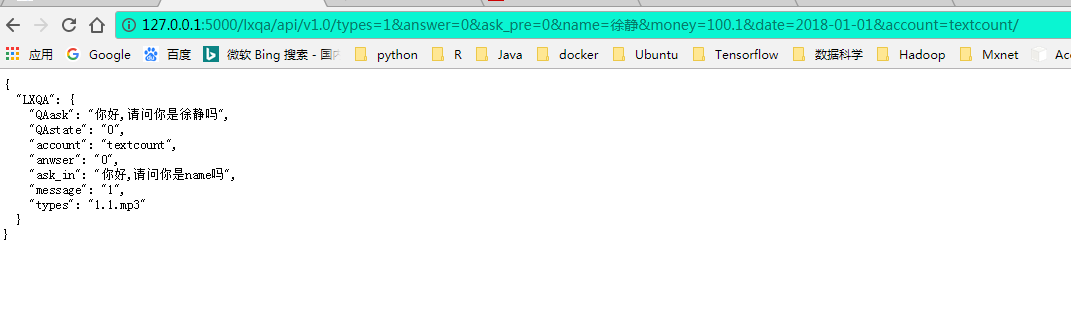
\includegraphics[width=1.5\linewidth,height=1.5\textheight]{img/2-1} \end{center}

\begin{itemize}
\item
  QAask: 当前自呼机器人的表述
\item
  QAstate:
  当前自呼机器人的是否挂断的判断:``0''表示不挂断,``1''表示挂断,结束通话
\item
  account: 债务人的账户
\item
  answer: 债务人上一轮的表述
\item
  ask\_in:
  当前聊天机器人的话术模板,作为下一轮调用自呼机器人的ask\_pre参数取值(GET请求时,ask\_pre字段应该提交聊天机器人的话术)
\item
  identity:
  债务人身份确认,可能性的取值有:0(当前无法判断),本人,其他联系人,异主
\item
  message: API调用的状态,``0''表示调用API异常,``1''表示调用API正常
\item
  types: 返回聊天机器人对用的音频文件
\end{itemize}

Example2:聊天过程中的调用,此时存在answer和ask\_pre字段,此时需用传入真实的字段文本内容,此时的URL为:

\begin{verbatim}
http://ip:port/lxqa/api/v1.0/types=1&answer=不是啊&
  ask_pre=你好,请问你是name吗&money=100.1&date=2018-01-01&account=textcount/
\end{verbatim}

\begin{center}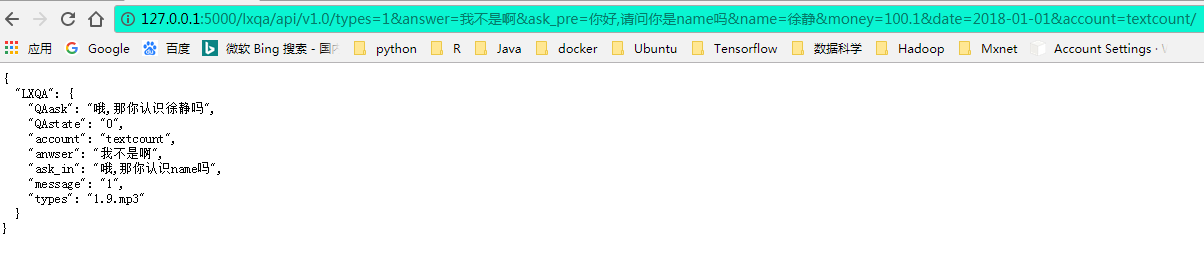
\includegraphics[width=1.5\linewidth,height=1.5\textheight]{img/2-2} \end{center}

返回的JSON字段意义同Example1中,但要注意,在过程中GET请求的数据一定要填写answer和ask\_pre字段,并且ask\_pre字段的是聊天机器人的话术模板,而非真正的ask字段。

\section{\texorpdfstring{\textbf{调用方式}}{调用方式}}

可以通过Java,Python,R语言等工具,通过GET请求访问并实时获取API的数据。

\chapter{返回Audio的API}\label{audio-api}

我们除了提供了JSON字符串格式的API之外,还提供了音频返回的REST
API,该API接口除了返回标准的JSON字符串之外,还额外的返回了,当前自呼机器人聊天的语音文本(语音格式是.mp3),基于GET请求中types参数的变化(1types=1:温暖女法务版,types=2:专业男法务版;types=3:专业男法务磁性版),
类似于百度云语音中的TTS REST
API接口支持语音的在线试听和下载。目前该API接口仅支持GET请求。

\section{\texorpdfstring{\textbf{GET请求的格式}}{GET请求的格式}}\label{get-1}

\begin{verbatim}
http://ip:port/lxqa/api/v1.0/audio/types=<types>&answer=<answer>&ask_pre=<ask_pre>
        &name=<name>&money=<money>&date=<date>&account=<account>/
#注意与JSON API的区别
\end{verbatim}

\begin{itemize}
\item
  ip:ip地址,具体的联信商务咨询有限公司会提供
\item
  port: 端口号,具体的联信商务咨询有限公司会提供
\item
  types:
  发声人,目前我们提供了三个发声人types=1:温暖女法务版,types=2:专业男法务版;types=3:专业男法务磁性版
\item
  answer: 上一轮债务人的反应对应的文本
\item
  ask\_pre:上一轮联信自呼机器人的话术模板
\item
  name: 债务人的姓名
\item
  identity:
  债务人身份确认,可能性的取值有:0(当前无法判断),本人,其他联系人,异主
\item
  money:债务人对应的委案金额
\item
  date:接单时间
\item
  account:账户
\end{itemize}

\section{\texorpdfstring{\textbf{举个栗子:}}{举个栗子:}}\label{-1}

Example1:开始拨打电话,此时并没有answer和ask\_pre字段,此时需用``0''填补这两个字段,此时的URL为:

\begin{verbatim}
http://ip:port/lxqa/api/v1.0/audio/types=1&answer=0&ask_pre=0&
      name=徐静&money=100.1&date=2018-01-01&account=testcount/
\end{verbatim}

\begin{itemize}
\item
  types=1:调用温暖女法务版机器人
\item
  answer=0和ask\_pre=0:
  因是第一轮对话,没有answer和ask\_pre因此传入参数``0''
\item
  name=徐静:债务人的姓名叫徐静
\item
  money=100.1:债务人的欠款金额是100.1
\item
  date=2018-01-01:
  债务人的案件的接单时间是2018年01月01日(注意该格式可以是任意类型的时间字符串)
\item
  account=testcount: 债务人对应的系统账户为testcount
\end{itemize}

此时GET请求将会返回如下的JSON字符串

\begin{center}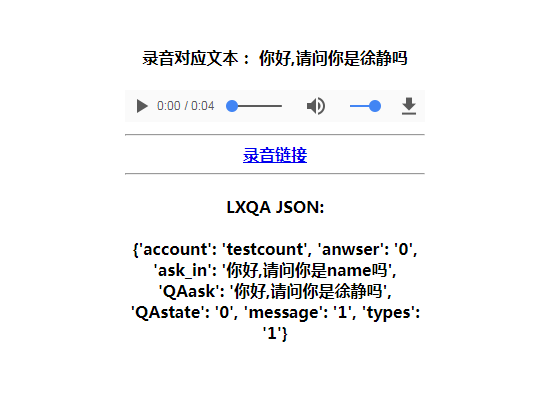
\includegraphics[width=1.5\linewidth,height=1.5\textheight]{img/3-1} \end{center}

录音对应文本:当前自呼机器人的返回内容

录音链接:下载录音的地址

LXQA JSON 同第二章相同:

\begin{itemize}
\item
  QAask: 当前自呼机器人的表述
\item
  QAstate:
  当前自呼机器人的是否挂断的判断:``0''表示不挂断,``1''表示挂断,结束通话
\item
  account: 债务人的账户
\item
  answer: 债务人上一轮的表述
\item
  ask\_in:
  当前聊天机器人的话术模板,作为下一轮调用自呼机器人的ask\_pre参数取值(GET请求时,ask\_pre字段应该提交聊天机器人的话术)
\item
  message: API调用的状态,``0''表示调用API异常,``1''表示调用API正常
\item
  types: 返回聊天机器人对用的音频文件
\item
  identity:
  债务人身份确认,可能性的取值有:0(当前无法判断),本人,其他联系人,异主
\end{itemize}

Example2:聊天过程中的调用,此时存在answer和ask\_pre字段,此时需用传入真实的字段文本内容,此时的URL为:

\begin{verbatim}
http://ip:port/lxqa/api/v1.0/audio/types=1&answer=不是啊&
  ask_pre=你好,请问你是name吗&money=100.1&date=2018-01-01&account=textcount/
\end{verbatim}

\begin{center}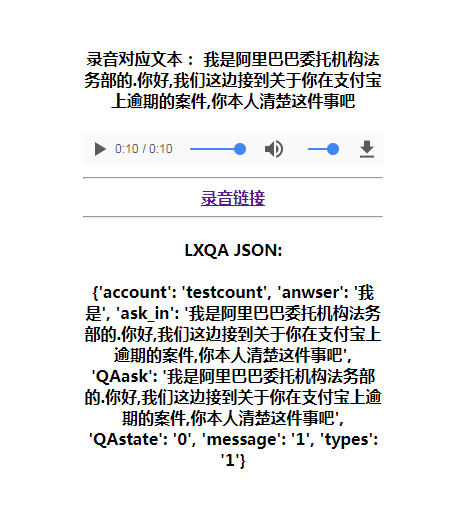
\includegraphics[width=1.5\linewidth,height=1.5\textheight]{img/3-2} \end{center}

返回的JSON字段意义同Example1中,但要注意,在过程中GET请求的数据一定要填写answer和ask\_pre字段,并且ask\_pre字段的是聊天机器人的话术模板,而非真正的ask字段。

\section{\texorpdfstring{\textbf{调用方式}}{调用方式}}\label{-1}

可以通过Java,Python,R语言等工具,通过GET请求访问并实时获取API的数据。

\bibliography{book.bib,packages.bib}


\end{document}
